\chapter{Carving: Finding Hidden Files in Bulk Data}












\color{red} 
Overall comments:

1 - This is great start. Remember that it's coming after the chapter
that describes disks and file systems (\chapref{ch-drives}) and the
chapter on finding hidden information in file systems
(\chapref{ch-fshidden}). In \chapref{ch-drives} we show people how to
work with disk images; in \chapref{ch-fshidden} we show how to use
SleuthKit to recover deleted files. I want \chapref{ch-fshidden} to
end with the idea that there are all these data that can't be
recovered because we don't have file system metadata. This chapter
will introduce traditional header/footer carving, carving with
validation, fragment recovery carving, and hash-based carving.

\color{black}










\emph{File carving} (also called \emph{data carving} or simply
\emph{carving}), is a digital forensics technique used to recover
files, file fragments, or other kinds of objects based on their
structure or content, rather than using metadata. Carving is a
critical technique in privacy auditing because it can find data that
are present and usable, but are invisible because pointers to the
data have been erased.

Most carvers will operate on any block of data of any size. It's
common to use carvers to search for data in disk images. But carvers
can be used to search other kinds of data as well. For example, you
can run a carver on a database file to see if information is present
in the file that cannot be retrieved through the database API.
(\citeN{1247492} demonstrated how MySQL left significant information
in database table storage, the transaction log, indexes, and other
system components.) Carvers can be applied to other data streams as
well, including physical memory (or memory images), and even network
packet captures.

File carving is a powerful tool for recovering data when filesystem
metadata (e.g., directory structures) is corrupt or destroyed, which
occurs when old files have been deleted or the data source is
corrupted, e.g., if data is being recovered from a damaged hard drive.
When file carving is applied to traditional non-volatile storage
media, such as hard drives, solid state drives, or removable media
such as USB thumbdrives, the objects to be recovered are usually
documents (e.g., Microsoft Word or PDF files), images (e.g., JPEG or
PNG-format graphics files), video files (e.g., AVI or MPEG format
movies), or other common file types.  For physical memory carving,
recovered objects are generally operating systems kernel or
application data structures, which can reveal the current or
historical state of a computer system.


\begin{figure}[ht]
\begin{center}
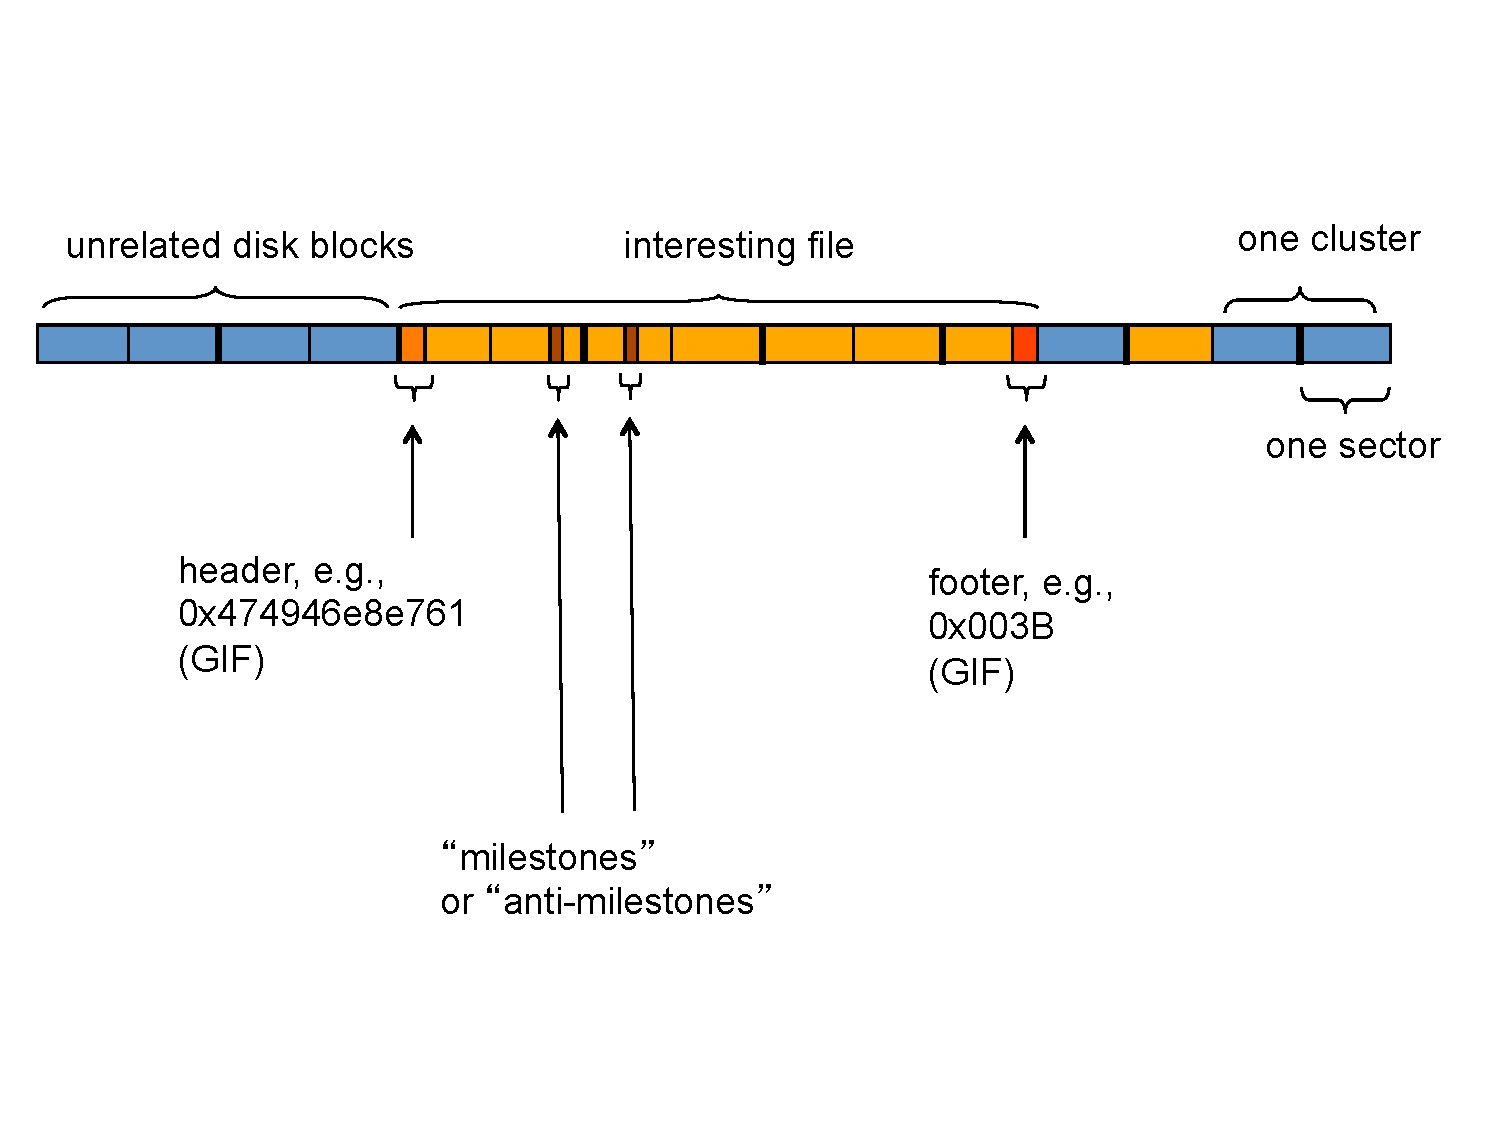
\includegraphics[width=140mm]{ch-carving/carvingoverview.pdf}
\end{center}
\caption{A high level overview of file carving.  A file carver
  searches for binary strings called headers that mark the beginnings
  of relevant file types.  Other data is then evaluated to determine
  where the file ends and potentially, for validation.  The figure
  illustrates an ideal situation$-$difficulties arise when unrelated
  data blocks intervene between the header and footer as a result of
  file fragmentation, or in more serious cases, when the fragmentation
  results in the header and fooger being in reverse order.  Files may
  also be partially corrupted, resulting in, e.g., a missing footer.}
\label{fig:carvingoverview}
\end{figure}

Historically, file carvers operated by looking for file headers and
footers, which are unique strings of bytes that appear at predictable
places near the beginning and end of files of a particular type
\cite{Foremost, Scalpel}, as depicted in Figure \ref{fig:carvingoverview}.
Such sequences are sometimes called
\emph{magic numbers.} Carvers may also scan for \emph{milestones}, which
are other strings of bytes that intervene between the beginning and
end of the file, to attempt to eliminate false positives 
\label{def:milestones}.  Carving programs often have an option to look for headers
only at or near sector boundaries, because files are almost always
created on a sector boundary.  However, searching the entire input
without regard to sector boundaries can enable discovery of embedded
files, such as JPEGs embedded in Microsoft Word or in archives
(e.g. ZIP files).  Depending on the circumstances, this may be either
an advantage or disadvantage. 

While header/footer--based file carving is still widely used to
recover data from storage media, other carving strategies have been
developed, to increase the accuracy of file carving tools by
incorporating detailed knowledge of specific file types and validation
mechanisms, and to expand the scope of carving to other types of
media.  Recent research has also concentrated on improving the
performance of carving tools and whereas carving was once a fairly
time--intensive process, data recovery using carving can now generally
be performed at the rate that the target storage media can transfer
data.  There has also been some limited success in developing tools
that can handle fragmented objects, but these are generally limited to
recovery of specific file types and the majority of carving tools
cannot automatically reconstruct arbitrarily fragmented
objects. 

\color{red}

RE below, any idea on how to structure the presentation in a figure / box?
\hl{mention fragment recovery carving and hash-based carving. We should probably have the
  carving taxonomy in a box. Each of these approaches should be
  described below?}
\color{black}

Applications of file carving and more details about the various file carving techniques currently in use are presented below.

\section{Using Carving to Find Hidden Data}

Carving is typically used to recover objects or object fragments (most
commonly, files or file fragments) that have been deleted.  Carving
might be carried out to support a digital forensics investigation, in
the context of criminal or civil litigation, during incident response,
or to recover data that's been inadvertently lost, e.g., as a result
of corrupted media or user error.  For the purposes of privacy
auditing, carving can be used in precisely the same manner it would be
used in a digital forensics investigation of broad scope--namely, to
determine what sensitive data can be recovered from target media.  For
example, most modern operating systems delete files by simply
modifying filesystem metadata to free resources such as inodes or MFT
entries and the data blocks allocated to the files.  This makes the
files ``disappear'' from a user's view, without actually scrubbing the
data blocks previously allocated to the file.  These data blocks then
reside in the unallocated regions of storage media, inaccessible to
most users, until they are allocated to new files and overwritten.

There are numerous situations where this shallow file deletion process
exposes sensitive user data to recovery.  For example, when users
clear web browser caches, empty the recycle bin on Microsoft Windows
systems, clear system logs, or delete files from the command line,
typical users lose \emph{control} over potentially sensitive data, but
the data is often easily recovered with carving techniques.
Furthermore, there are situations where operating systems allocate
significant amounts of disk space on a semi-permanent basis without
sanitization, resulting in data being trapped (and recoverable via
file carving) for long periods of time.

Consider, for example, the HTML fragment and image file depicted in
Figure \ref{fig:insideswapfile}, which were carved from a Windows XP
swap file.  Because of the structure and organization of swap files,
it would be very unusual for this data to be present as a result of
swapping--in fact, in this case, the two deleted files were trapped
when Windows extended the swap file, and were easily recovered using
file carving.  Another common misconception is that format operations
permanently destroy data.  In fact, with the exception of how SSDs are
handled in recent versions of modern operating systems, most format
operations destroy little data.  In figure \ref{fig:formatting}, the
effects of formatting a 256MB thumb drive for three different
filesystems is depicted.  Even after the third format operation, most
data remains.  These visualizations were generated using the Python program
shown in Listing~\ref{vizdiff}, based on an old Perl script written years again, and works
under both Python 2.7 and 3.3+. 

\lstinputlisting[caption=A simple Python program for visualizing the differences
between a series of identically sized disk images,label=vizdiff]{ch-carving/vizdiff.py}

The thumb drive stored four photographic images in
addition to a variety of other files.  All four photographic images
stored on the thumb drive were still completely recoverable after the
format operations, as illustrated in Figure \ref{fig:recovered}.

\begin{figure}[ht]
\center
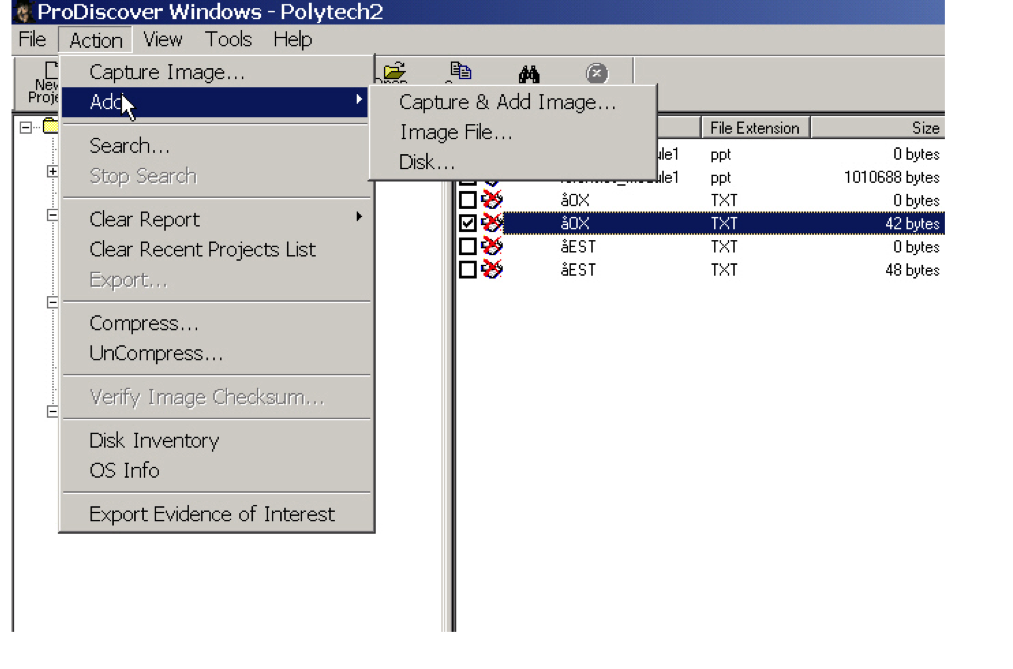
\includegraphics[width=100mm]{ch-carving/imageinswap.png}
\vspace{3mm}
\noindent\rule{60mm}{1pt}
\vspace{3mm}
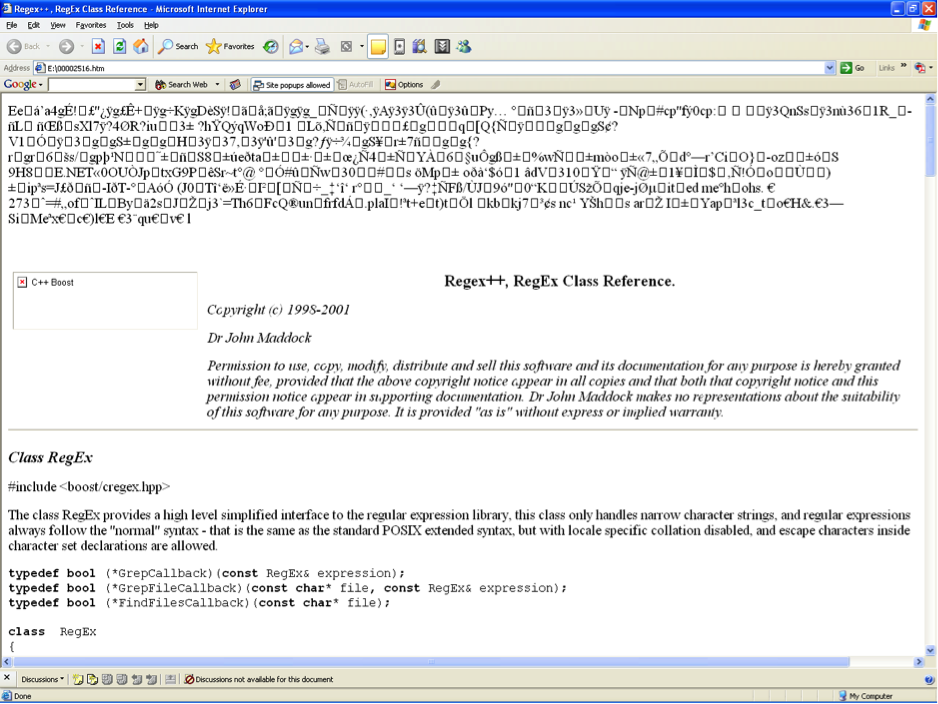
\includegraphics[width=100mm]{ch-carving/cacheinswap.png}
\caption{Image file and HTML fragment carved from a Windows swap file.  These are deleted documents ``trapped'' in the un-sanitized space allocated by Windows to the swap file.}
\label{fig:insideswapfile}
\end{figure}

\begin{figure}[ht]
\centering
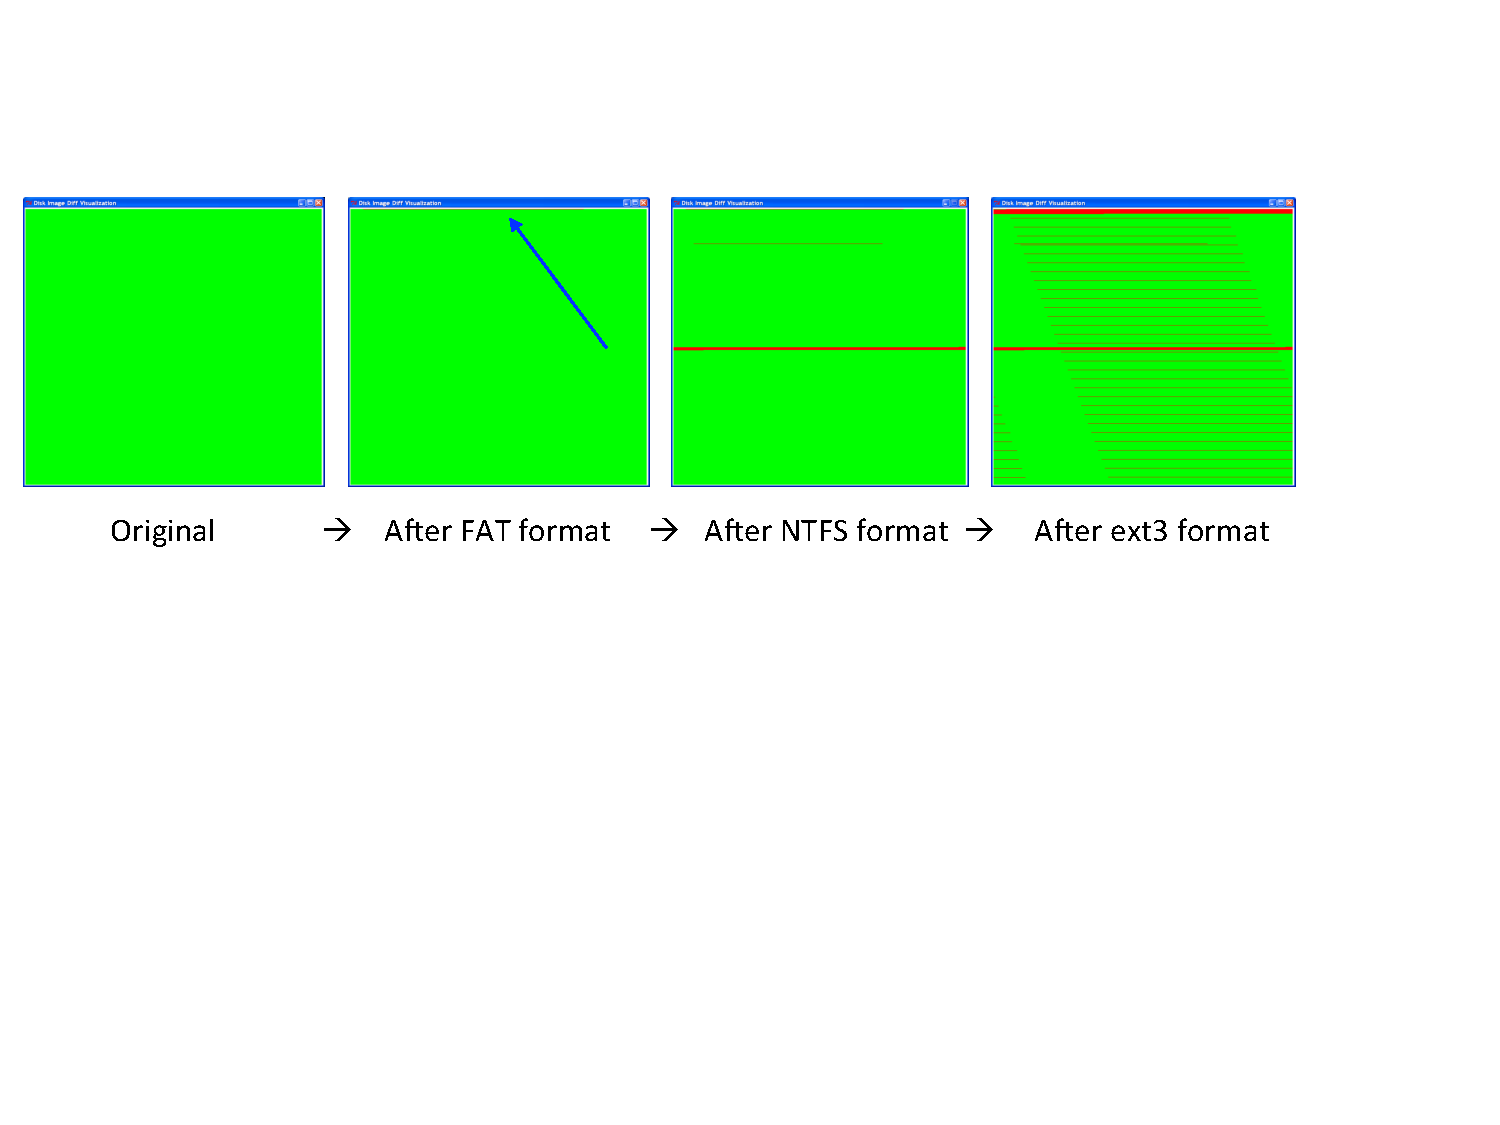
\includegraphics[width=150mm]{ch-carving/formatting.pdf}
\caption{Illustration of the effects of formatting on a 256MB thumb drive.  As the thumb drive is formatted for different filesystems, a small amount of data is lost (depicted in red), but the vast majority of data remains even after three different format operations.}
\label{fig:formatting}
\end{figure}


\begin{figure}[ht]
\centering
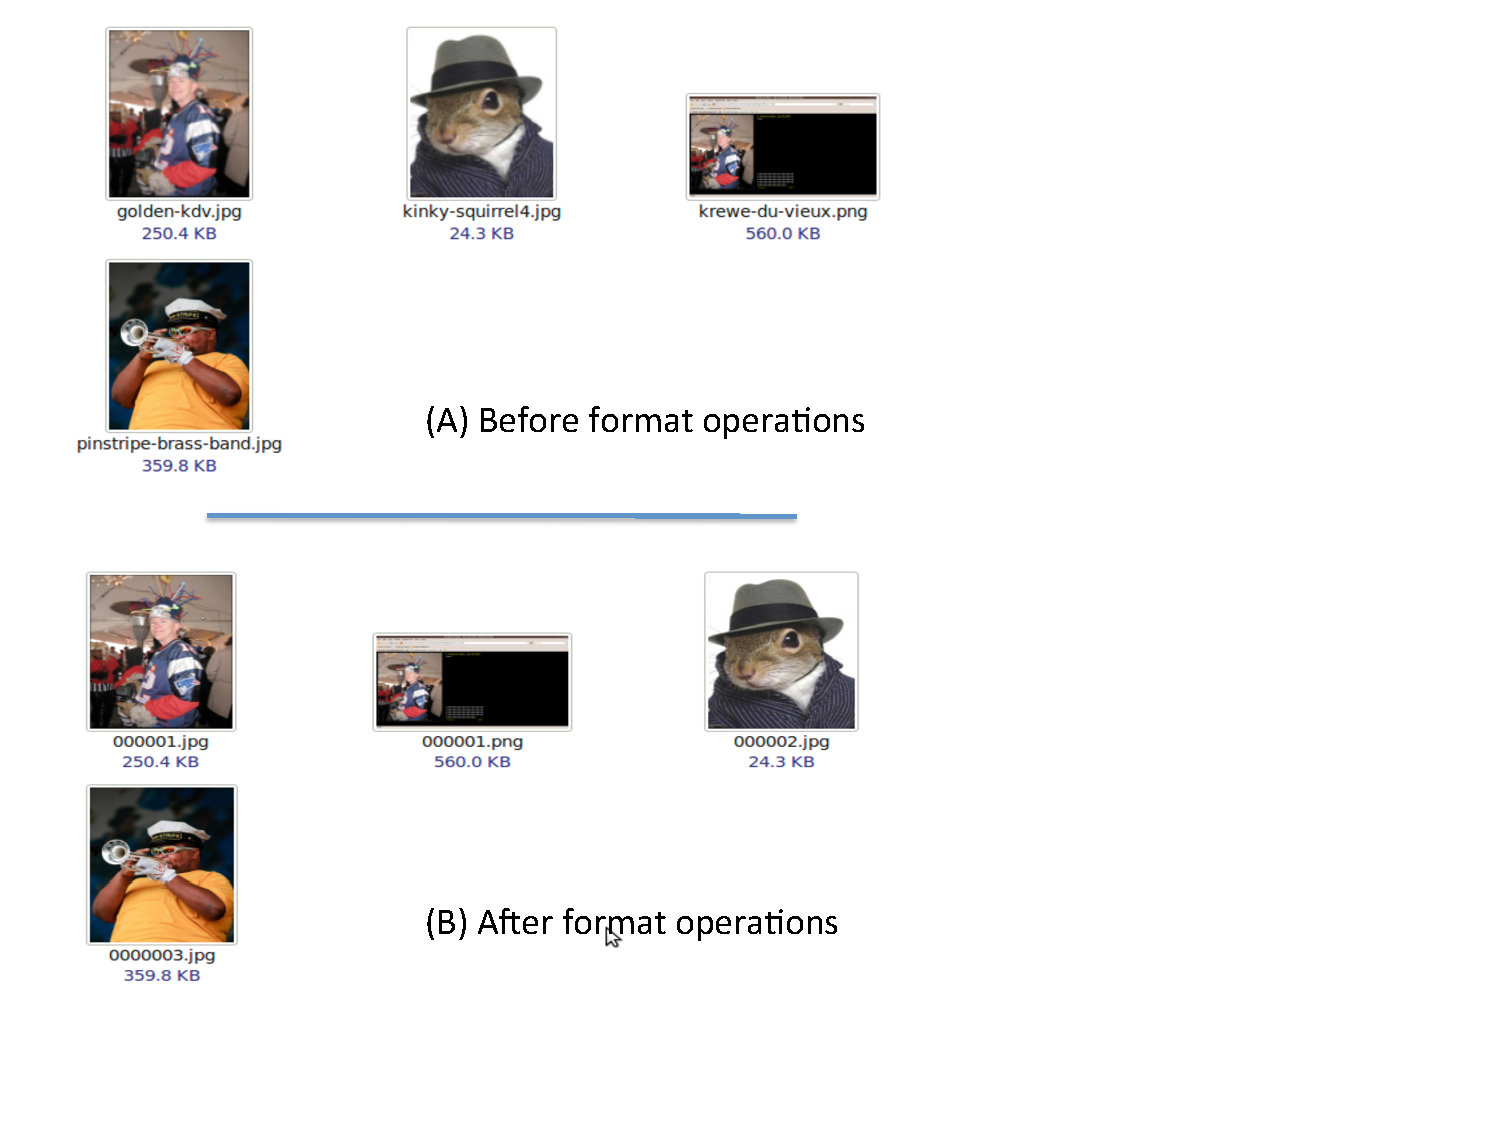
\includegraphics[width=150mm]{ch-carving/recovered.pdf}
\caption{Four photographic images stored on the thumb drive, depicted in (A), are completely recoverable as shown in (B), even after the format operations described in Figure \ref{fig:formatting}.  Only the associated filenames are lost.}
\label{fig:recovered}
\end{figure}


Given that carving can recover data that is otherwise completely inaccessible to non-technical users, it is imperative that privacy advocates understand the capabilities and limitations of this forensic technique.  


\section{How Carvers Work}
In this section we will discuss the specifics of how carvers work. We
will look at three carvers: scalpel, a traditional carver; PhotoRec, a
modern carver with a pluggable architecture; and frag\_find, a
hash-based carver.

\subsection{Header/Footer\-Based Carving with Scalpel}

Header/footer based carving tools use a database of carving rules,
with each rule defining how objects of a particular type should be
identified in a data stream. This approach is similar to that used by
the Unix {\tt file} command, which uses a database of rules to
identify file types.  For carving, the rules help to identify the
starting and ending locations of files a stream, and allow the carving
tool to copy sequences of bytes between the header and footer into
regular files for examination. A rule typically defines a header and
optionally, a footer, each of which is a binary string expected to be
discovered near the beginning/end of objects of the corresponding
type.  For example, for JPEG file types, the appropriate header is
0xFFD8FFE00010 and the footer is 0xFFD9.  The rule also commonly
provides other guidance to the carving tool, including the minimum and
maximum sizes of matching objects that should be carved, whether
alphabetic components of the header and footer are case sensitive, and
whether carving operations for an object should cease if the header of
a matching object is encountered (this identifies objects stored "back
to back" on the storage media).  Other guidance to the carving tool
might include whether to choose the footer closest to a discovered
header or farthest away from the header, and whether the footer should
actually be included in the recovered object.  To illustrate some of
these issues, consider the following carving rules from a
configuration file for Scalpel \ref{Scalpel}, a popular
header/footer--based file carver:

{
% SLG commented out \medium, as it caused a problem
% \medium
\begin{Verbatim}
  # image files: GIF, JPG, PNG
  gif  y   100:500000   \x47\x49\x46\x38\x39\x61 \x00\x00\x3b
  jpg  y   1000:8000000 \xff\xd8\xff\xe0\x00\x10  \xff\xd9
  png  y  1000:5000000  \x50\x4e\x47?  \xff\xfc\xfd\xfe
  #
  # Legacy Microsoft Office documents
  doc  y  1000000      \xd0\xcf\x11\xe0\xa1\xb1\x1a\xe1\x00\x00 
  # Illustration of regular expression-based headers and footers
  xyz  y   100000  /GGG[^G]/    /[0-9]HHHHH/
\end{Verbatim}
}

Comments in the example above begin with a hash mark ("\#") and are
ignored by the carving tool.  The first rule carves GIF format images
files, and used "gif" as the extension for recovered files.  The "y"
indicates that the header and footer and are case-sensitive.
"100:500000" indicates that only files between 100 and 500,000 bytes
(inclusive) should be recovered.  The final two elements of the rule
are the header and footer, represented by hexadecimal strings.  The
JPEG and PNG rules are similar.  The Microsoft Office rule is
different, in that no footer is specified.  In this case, files that
match the header are carved to the maximum size specified (in this
case, 1,000,000 bytes).  Rules like this are wasteful of space, but if
file types don't have strings that can be reliably predicted to be
near the end of file, then for header/footer--based carving, there's
essentially no choice.  The final rule illustrates
header/footer--based carving being used to carve objects with headers
and footers specified by regular expressions.  In this rule, files of
a maximum of 100,000 bytes are carved if they begin with a string of
three "G" characters, followed by a character other than a "G".  The
file is terminated by a digit (0--9) followed by five "H" characters.
Using regular expressions for headers and footers potentially
decreases performance of the carving tool, but provides a much more
powerful means to describe the objects to be recovered.  Creating a
new rule can be time--consuming, because some knowledge about the
common structure of files of the new type is required, but this
knowledge need not be nearly as deep as for \emph{semantic carving},
covered later in the chapter.

One benefit of header/footer-based carvers is that they can retrieve
files from a raw disk image in a filesystem--agnostic way, operating
regardless of the type of filesystem on the disk image.  Perhaps more
importantly, file carving is possible even if the filesystem metadata
has been destroyed, such as during a filesystem format operation or as
a result of file corruption due to media damage, a power outage, or
similar event.  One limitation of header/footer--based carving tools
is that an object's data must be contiguous to be carved properly.
With manual intervention or multiple carving steps which prune out
previously recovered objects from the target media, some
non-contiguous objects can be recovered, but in general fragmented
objects are problematic.  Still, header/footer--based carvers that
encounter fragmented objects can still partially recover the objects,
and even object fragments may pose significant risks to privacy.
Finally, of the various types of file carvers, header/footer--based
carvers are generally the most configurable, since only the binary
strings that delimit the beginning and end of targeted file types must
be described.  In contrast, deep carvers, which have extensive
knowledge of the format of specific file types, generally require
writing code to target additional file types.

\subsection{Reducing False Positives with PhotoRec, a Semantic Carver}

Unlike header/footer-based carving, \emph{semantic} or \emph{deep
  carving} uses detailed knowledge of individual file types to detect,
parse, and recover files from disk images or raw, physical disk
devices.  Whereas header/footer-based carving uses only minimal
structural information about particular file types, the goal of
semantic carving is to leverage sufficient information about
particular file types to allow more accurate detection and validation
of files (thus reducing false positives).  Semantic file carvers also
attempt to use file metadata to determine the precise lengths of files
to be recovered, reducing "over-carving", which results frequently
when header/footer-based carvers cannot accurately determine where a
file ends.  Semantic carving is much more resilient in carving
compound files, e.g., files that contain other files (examples include
archives such as ZIP, but also image files with embedded thumbnails,
to support rapid previewing).  Since the semantic file carver
understands the structure of the container file, embedded files such
as thumbnails can simply be included without further processing by the
carver, preserving the integrity of the compound file.  Header/footer
based carving tools like Scalpel include experimental features that
try to correlate nested headers and footers (e.g., in the case of an
image file with embedded thumbnails), but in practice these cases are
better handled with deeper knowledge of the structure of files of
particular types.

Early attempts to reduce false positives in file carving introduced
validators, which performed consistency checks to determine the
validity of recovered files (e.g., decompressing a recovered JPEG file
to determine if it decompresses properly, or analyzing the format of a
ZIP file to see if the archive is intact).  Files that fail validation
can either be discarded or marked as corrupted, but preserved for
deeper examination by an investigator.  Photorec \cite{photorec} is
currently the state-of-the-art semantic carver, supporting more than
400 file types.  Attempts to recover individual file types in Photorec
are triggered by discovery of a matching header in a disk image.
Execution of file type-specific C functions (written by the author of
the tool or by investigators wishing to extend the list of types
supported by Photorec) follow the discovery of the header, and these
functions validate the data as well as parse relevant file metadata to
discover the length of the file and other information.  For example, the file
|file_jpg.c|, part of the source code for Photorec, deals with validation of 
JPEG images and incorporates a number of checks to ensure that JPEG
files are properly carved.  This detailed
knowledge of file structures greatly increases accuracy when carving
pristine files, but it can be time-consuming to accommodate new file
types due to limited documentation of their formats and generally
requires programming skill.

\subsection{The challenge of fragmented files}

Dealing with fragmented objects is the most difficult problem in
carving.  In legacy filesystems such as FAT, which does not
incorporate strategies to reduce file fragmentation, many small files
are likely to be stored contiguously, because files are created on
cluster boundaries and cluster sizes under FAT tend to be rather
large.  Larger files on FAT filesystems, however, are commonly
fragmented\cite{dfrws2007:SimsonLGarfinkel}.  While modern filesystems
such as NTFS, ext2/3/4 and HFS+ do take steps to ensure that
fragmentation of files is reduced, fragmentation does still occur.
Furthermore, performance for SSDs does not benefit from legacy
anti--fragmentation mechanisms, and some of these mechanisms may
actually reduce SSD lifespan.  As a result, some anti--fragmentation
strategies are suppressed when SSDs are in use.  

While some tools
exist for recovering fragmented files of certain types \cite{adroit},
a general approach for fragmented file recovery is considered intractable.
For a special case, however, when a copy (or partial copy) of a file to be
recovered is available, \emph{hash--based carving} can be used to discover
even highly fragmented files.  This is useful in establishing the existence
of known files on a disk image, in contrast to the discovery of unknown
files.  Hash-based carving is covered in the next section.

\subsection{Hash-based carving with frag\_find}

The frag\_find carver uses sector hashes to search for parts of a target file, called the \emph{master file}, in a disk image. Hash-based file carvers are particularly useful for establishing that copies of the master file exist (or existed) on the disk image.  Since files in commonly used filesystems are always fragmented on boundaries that are a multiple of the hard drive's sector size, sectors belonging to even highly fragmented copies of the master file on the disk image are easily discovered.  frag\_find works as follows:

\begin{itemize}

\item First, for each master file, a data structure is created that can map each master file sector to a set of sectors in the image file. This data structure is called a \emph{filemap} and one is created for each master 
file.

\item Every sector of each master file is scanned. For each sector in the file, both the MD5 and SHA-1 hashes are computed. Each MD5 hash is used to set a corresponding bit in a Bloom filter. The
SHA-1 hashes are stored in a data structure called the \emph{shamap} that maps SHA-1 hashes to one or more sectors in the master file.  

\item Each sector of the disk image is scanned. For each sector, the MD5 hash is computed and the corresponding bit checked in the Bloom filter.  If the sector’s MD5 is found in the Bloom filter, then 
the sector’s SHA-1 hash is calculated and the \emph{shamap} structure is examined--for each matching sector found in the \emph{shamap}, the sector number of the matching sector in the disk image is added to the corresponding sector in each \emph{filemap}.  This allows frag\_find to track the locations in the disk image that match fragments of each master file. 

\item Each \emph{filemap} is then scanned for the longest runs of consecutive sectors in the disk image.    This run is noted and then removed from the \emph{filemap}. The process is repeated until the \emph{filemap} is empty.  The goal of this step is to identify the largest contiguous chunks of a master file that appear in the disk image, since the presence of large chunks of the file is highly indicative of the file previously existing in the disk image.

\end{itemize}

The likelihood that matching sectors discovered by frag\_find are correlated with master files being  previously stored in the disk image depends on several factors.  First, \emph{distinct sectors}, that is sectors that are manufactured by some random process, like the sectors comprising the compressed image data in a JPEG of a desert flower, are very likely to be unique to a particular file. Confidence that sectors are distinct can be strengthened by searching for them in a large disk corpus and verifying that they are found only in the master file and nowhere else.  Thus, for distinct sectors, matching even a single sector between a master file and disk image is a strong indicator that the file previously existed on the disk.  Second, the presence of large contiguous runs of sectors, particularly distinct sectors, is even stronger evidence that a master file previously existed on the disk.


\section{Memory Carving}

\hl{In this section, perhaps a simple example of memory carving to
  show how relatively short structured information can be readily
  recovered. My suggestion is to discuss the carving of some Windows
  data structure that is easy to validate and contains significant
  private information, such as a process list or a network packet
  (IPv4 header checksums do great validation here). We can use either
  Volatility or bulk\_extractor's code for discussion. Or both. }

USE VOLATILITY EXAMPLE HERE, e.g., command console stuff?


\begin{Verbatim}
Physical memory acquisition, Volatility, maybe specialized, standalone
stuff, but most of that functionality is making its way into
Volatility anyway, better in general to carve against virtual address
spaces so things are contiguous, et al
\end{Verbatim}


\color{red}
Decide where (if at all) to talk about in-place carving, which can also be used to determine the locations (or simple existence) of recoverable objects, w/o the overhead of recovery
\color{black}



